\chapter{UAV Control}

\section{UAV visual-servoing controller using projective camera geometry}
This section introduces a relatively simple UAV control algorithm based on the projective camera geometry. We assume that the controller receives where target is in normalized image coordinate and camera is rigidly fixed to UAV platform. 

\subsection{Coordinate Frame Convention}
Before giving a detailed explanation of the control algorithm, it is worth clarifying our assumptions and the coordinate frames used in this section. 

First, an East-North-Up (ENU) coordinate frame is used as opposed to the common North-East-Down (NED) coordinates for UAV in order to match the frame convention used in the \texttt{mavros} package in ROS for hardware experiment. Let $\mathcal{F}^i$ be the inertial frame, which in this case coincides with the ENU frame, and let $\mathcal{F}^v$ be the vehicle frame that is translated to the UAV center of mass, with the same orientation as $\mathcal{F}^i$. Vehicle-1 frame, $\mathcal{F}^{v1}$ indicates the frame that is only rotated about the $z$-axis of $\mathcal{F}^{v}$ by $\psi$, the heading angle of the multirotor. The rotation matrix from $\mathcal{F}^v$ to $\mathcal{F}^{v1}$ can be expressed as $R^{v1}_v$. Other involved frames are optical, camera, and body frames expressed as $\mathcal{F}^o$, $\mathcal{F}^c$, $\mathcal{F}^b$, respectively. 

Second, a flat-earth model is used to properly scale the target position relative to the camera in $\mathcal{F}^{v1}$ and we have access to the correct altitude information. 

Third, the displacement between the center of mass of the UAV and the focal point of camera is ignored since it is negligible compared to the distance between the camera and the target. 

Fourth, we rely on GPS position controller on autopilot. The visual-servoing controller in this paper computes the desired multirotor position in order to follow the target and send the position command to the autopilot.

\subsection{Forward and heading motion control}
\begin{figure}[thpb]
	\centering
	\framebox{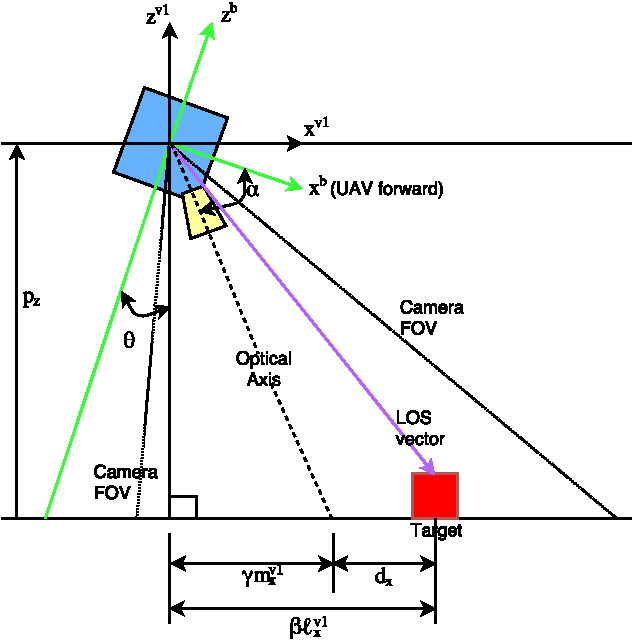
\includegraphics[width=4in]{images/side_view_45deg_2.pdf}}
	\caption{Side view of the multirotor.}
	\label{side_view}
\end{figure}
The first step of the motion control is to transform the line of sight (LOS) vector to the target in $\mathcal{F}^o$ into $\mathcal{F}^{v1}$. Let 
\begin{equation}
\mathbf{\ell}^o=[\epsilon_x^o, \epsilon_y^o, 1]^\top
\end{equation} where $\ell^o$ is the normalized line of sight vector in $\mathcal{F}^o$ and its third element 1 indicates the focal length of the camera in the normalized image. Let also the unit vector along the optical axis in $\mathcal{F}^o$ be defined as 
\begin{equation}
\mathbf{m}^o=[0, 0, 1]^\top.
\end{equation}
By applying sequential transformations to $\ell^o$ and $\mathbf{m}^o$, we get
\begin{equation}
\mathbf{\ell}^{v1}=R^{v1}_b(\phi,\theta)R^b_c(\alpha)R^c_o\ell^o=[\ell^{v1}_x, \ell^{v1}_y, \ell^{v1}_z]^\top
\end{equation}
\begin{equation}
\mathbf{m}^{v1}=R^{v1}_b(\phi,\theta)R^b_c(\alpha)R^c_o\mathbf{m}^o=[m^{v1}_x, m^{v1}_y, m^{v1}_z]^\top
\end{equation} where $R^b_c$ is a matrix with fixed values depending on how the camera is mounted with respect to $\mathcal{F}^b$, $R^{v1}_b$ is a matrix requiring the roll and pitch angles of the multirotor. The $\ell^{v1}$ is the displacement of the target relative to the multirotor and $\mathbf{m}^{v1}$ is the optical axis in $\mathcal{F}^{v1}$. The LOS vector $\ell^{v1}$ and $\mathbf{m}^{v1}$ do not have proper scalings due to the unknown depth information to the target in $\mathcal{F}^o$, but can be recovered using the altitude of the camera. Let
\begin{equation}
\beta=\frac{p_z}{\ell^{v1}_z}
\end{equation} 
\begin{equation}
\gamma=\frac{p_z}{m^{v1}_z}
\end{equation} where $p_z$ is the altitude of the multirotor. Then, the desired forward position from the current multirotor position can be computed as 
\begin{equation}
d_x=\beta\ell^{v1}_x-\gamma{m}^{v1}_x.
\end{equation}
This $d_x$ may be further broken down into east and north components
\begin{equation}
d_n=d_x\sin(\psi)
\end{equation}
\begin{equation}
d_e=d_x\cos(\psi)
\end{equation} where $\psi$ is the heading of the multirotor. These north and east components are added to the current multirotor east and north positions, and the sum is sent to the autopilot position controller.

It is more suitable to compensate for a target moving horizontally in the image plane by adjusting the multirotor's heading than through lateral motion. Thus, a yaw rate command $\omega_z$ can be computed as 
\begin{equation}
\omega_z=\eta \ell^{v1}_y,
\end{equation} where $\eta>0$ is a control gain.